\section{TECNOLOGIAS UTILIZADAS E BANCO DE DADOS}

Para materializar os pilares conceituais e operacionais do WeFIND apresentados no Capítulo 5, a seleção tecnológica priorizou ferramentas de comprovada maturidade técnica, suporte comunitário ativo e alta produtividade na escrita do código-fonte. Como orientam Pressman e Maxim (2021) e Valente (2023), a definição criteriosa da pilha de software (tecnologias clientes, serviços de nuvem e persistência de dados) constitui a base para assegurar desempenho, escalabilidade e manutenibilidade a longo prazo.

Este capítulo detalha as bibliotecas que compõem o ecossistema de desenvolvimento móvel do WeFIND, descreve a infraestrutura de computação em nuvem provida pelo Supabase, apresenta a modelagem lógica relacional do banco de dados PostgreSQL estruturada com políticas de segurança em nível de linha (RLS) e relaciona as ferramentas auxiliares utilizadas na gestão e governança do projeto.

\subsection{Tecnologias Utilizadas no Desenvolvimento Móvel}

A construção do aplicativo móvel exigiu a integração de ferramentas modernas voltadas à alta performance em smartphones. A Figura~\ref{fig:principais_tecnologias} destaca as principais tecnologias adotadas no projeto.

\begin{figure}[H]
    \centering
    \caption{Principais tecnologias que compõem o ecossistema WeFIND}
    \label{fig:principais_tecnologias}
    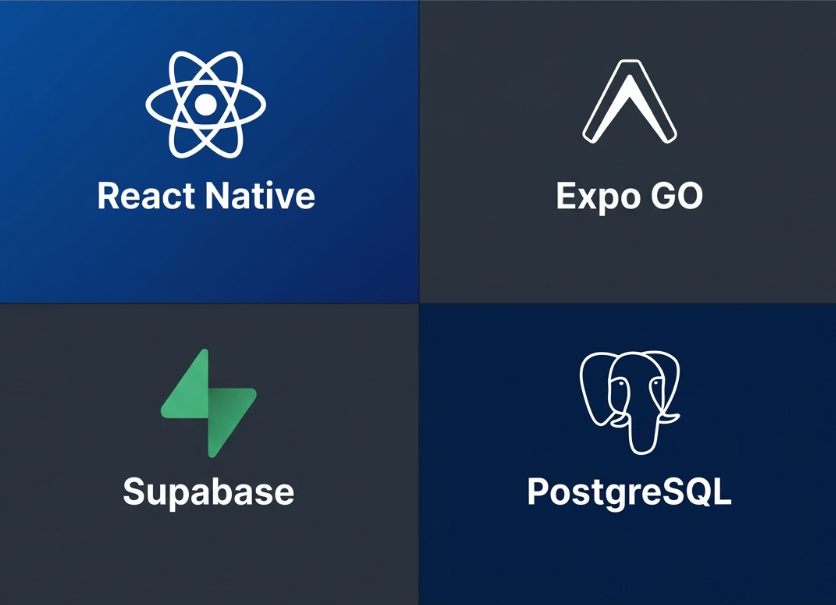
\includegraphics[width=0.90\textwidth]{imagens/03_arquitetura_design/figura11_principais_tecnologias.png}
    \fonte{Autoria própria (2026)}
\end{figure}

A biblioteca React Native (REACT NATIVE, 2026) foi adotada como núcleo para a interface móvel cliente. Sua principal vantagem reside na capacidade de compilar código nativo para as plataformas Android e iOS a partir de uma base unificada escrita em TypeScript e JavaScript. Essa estratégia reduziu substancialmente o ciclo de desenvolvimento e evitou a necessidade de manter projetos paralelos com linguagens distintas, garantindo consistência visual e facilidade de manutenção corretiva.

Em conjunto com o React Native, utilizou-se a plataforma Expo (EXPO, 2026). O Expo fornece um ecossistema abrangente de módulos nativos pré-configurados que simplificam o acesso aos sensores do smartphone. No WeFIND, o Expo foi fundamental para viabilizar a captura de coordenadas geográficas via pacote Expo Location, a seleção e captura de fotografias por meio do Expo Image Picker e a execução do aplicativo em dispositivos físicos durante as sessões de desenvolvimento.

Para resguardar o tráfego de rede e a integridade das consultas, foram inseridas regras de validação no próprio aplicativo cliente. Os formulários executam verificações em tempo real sobre campos de preenchimento obrigatório, validam a consistência de endereços de e-mail e realizam a redução e compressão automatizada de fotografias antes do upload para a nuvem, reduzindo o consumo do pacote de dados móveis do usuário.

\subsection{Serviços em Nuvem e Banco de Dados PostgreSQL}

Na camada de persistência e serviços em nuvem, selecionou-se a plataforma Supabase (SUPABASE, 2026). O Supabase atua no modelo de computação em nuvem integrado, fornecendo serviço de autenticação de usuários (Supabase Auth), armazenamento seguro de arquivos multimídia (Supabase Storage) e banco de dados relacional baseado em PostgreSQL, dispensando a complexidade de aluguel e manutenção de servidores dedicados.

O módulo Supabase Auth gerencia os fluxos de cadastro, login e redefinição de senhas, gerando chaves de autenticação em formato JWT (JSON Web Token) armazenadas de modo persistente no dispositivo móvel. Já o serviço Supabase Storage é responsável por hospedar os arquivos de imagem dos animais e dos perfis de usuário, servindo as fotografias por meio de links de distribuição pública de alta disponibilidade.

A persistência estruturada dos dados é realizada no sistema gerenciador de banco de dados relacional PostgreSQL. Para organizar de forma consistente as entidades, atributos e relacionamentos da plataforma, desenvolveu-se o modelo lógico relacional apresentado na Figura~\ref{fig:modelo_logico_banco}.

\begin{figure}[H]
    \centering
    \caption{Modelo Lógico Relacional do Banco de Dados PostgreSQL}
    \label{fig:modelo_logico_banco}
    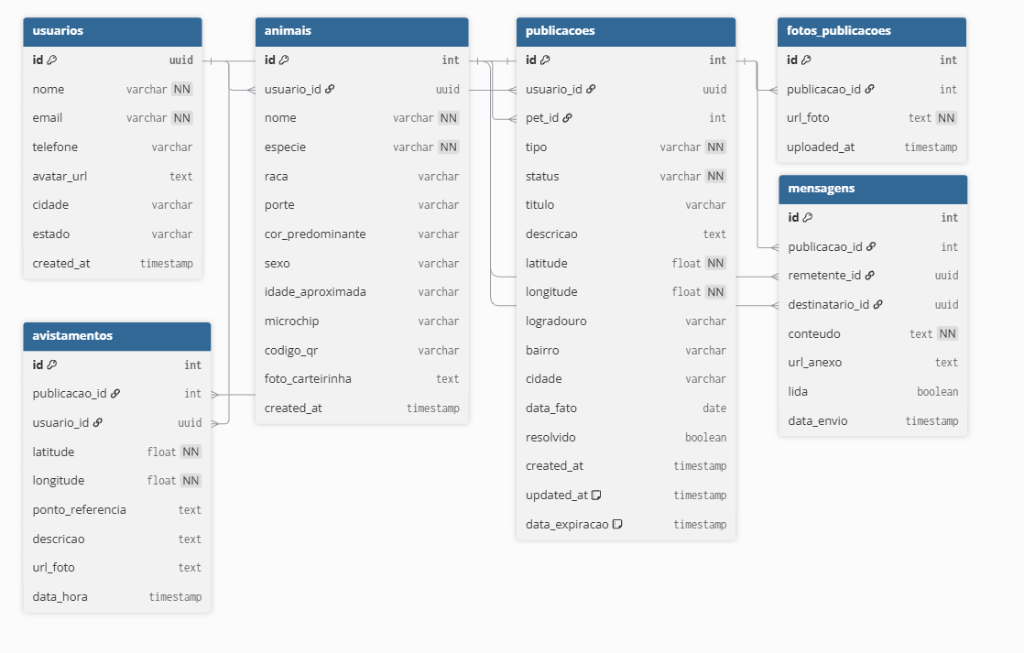
\includegraphics[width=0.92\textwidth]{imagens/02_modelagem/figura09_modelo_logico_banco.png}
    \fonte{Autoria própria (2026)}
\end{figure}

O modelo lógico da Figura~\ref{fig:modelo_logico_banco} é composto por cinco tabelas relacionais fundamentais:

A tabela \textit{usuarios} centraliza os dados cadastrais dos participantes do sistema. O campo identificador primário conecta-se diretamente à chave única fornecida pelo serviço Supabase Auth, registrando o nome completo, endereço de correio eletrônico, fotografia de perfil, número de telefone para contato emergencial, cidade, estado de residência e o registro de data e hora de criação da conta.

A tabela \textit{animais} armazena todas as ocorrências cadastradas na plataforma e estabelece chave estrangeira com a tabela \textit{usuarios}, identificando o autor da publicação. Entre os campos estruturados, constam o status operacional do registro (Perdido, Encontrado ou Adoção), nome do animal, espécie (canina ou felina), raça, porte físico, padrão de coloração da pelagem, sexo, faixa etária aproximada e indicador do uso prévio de coleira. Para possibilitar a busca espacial por proximidade e a plotagem exata no mapa interativo, a tabela armazena as coordenadas de latitude e longitude em formato de ponto flutuante, acompanhadas de campos descritivos para logradouro, bairro, município, data do fato, observações gerais e indicador de resolução do caso.

A tabela \textit{fotos\_animais} gerencia as fotografias anexadas a cada publicação, mantendo relacionamento de cardinalidade um-para-muitos com a tabela \textit{animais}. Essa estrutura armazena a URL pública da imagem persistida no armazenamento em nuvem do Supabase Storage, viabilizando o carregamento de múltiplas fotografias por anúncio com controle individual de exclusão.

A tabela \textit{avistamentos} organiza os relatos colaborativos fornecidos pela comunidade ao visualizarem animais soltos na rua. Cada registro vincula-se ao animal correspondente e ao usuário informante, armazenando as coordenadas de latitude e longitude do local exato do avistamento, ponto de referência descritivo, endereço textual aproximado, fotografia comprobatória opcional e carimbo de data e hora do relato.

Por fim, a tabela \textit{mensagens} dá suporte ao canal de comunicação privativo da aplicação. Ela reúne o identificador do animal em discussão, o identificador do usuário remetente, o identificador do usuário destinatário, o conteúdo textual da mensagem, anexo opcional de imagem, indicador booleano de confirmação de leitura e registro cronológico do envio.

A segurança e a integridade do banco de dados relacional são asseguradas por políticas de segurança em nível de linha (Row Level Security, ou RLS). Por meio desse mecanismo, implementado diretamente no mecanismo do PostgreSQL, define-se que qualquer usuário autenticado ou visitante possui permissão de leitura sobre as publicações de animais ativos, porém apenas o usuário proprietário daquele registro detém privilégios para alterar ou excluir suas próprias publicações e dados de perfil, impedindo modificações não autorizadas.

\subsection{Ferramentas Auxiliares de Apoio}

Durante as etapas de planejamento, especificação, escrita de código e desenho visual, recorreu-se a um conjunto de ferramentas auxiliares de apoio ao desenvolvimento, ilustradas na Figura~\ref{fig:ferramentas_auxiliares}.

\begin{figure}[H]
    \centering
    \caption{Ferramentas auxiliares de apoio ao desenvolvimento do projeto}
    \label{fig:ferramentas_auxiliares}
    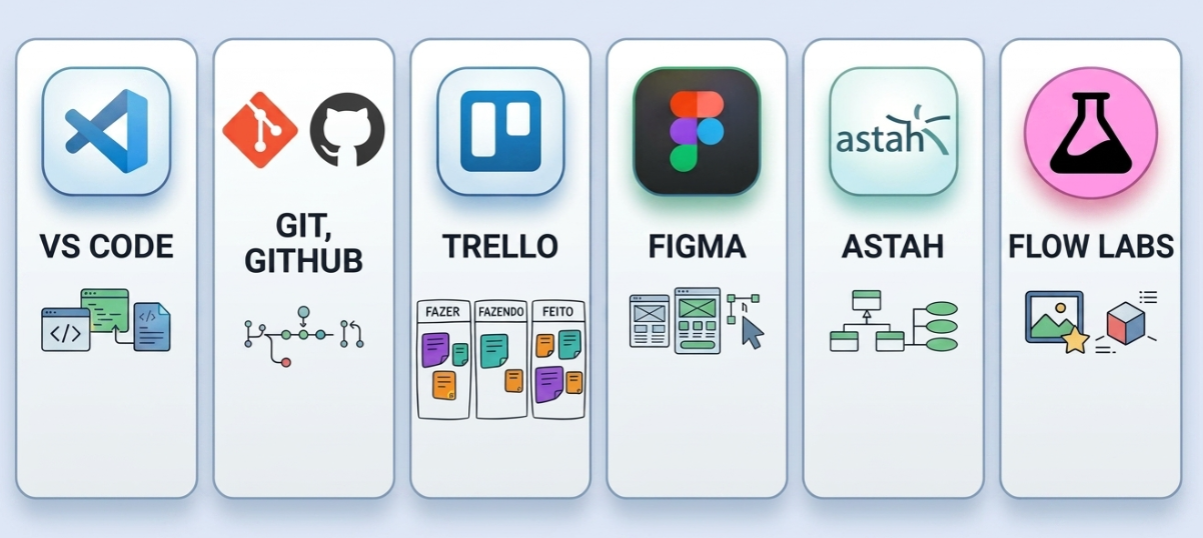
\includegraphics[width=0.90\textwidth]{imagens/03_arquitetura_design/figura12_ferramentas_auxiliares.png}
    \fonte{Autoria própria (2026)}
\end{figure}

A escrita, compilação e depuração do código-fonte foram conduzidas no editor Visual Studio Code (VS Code), com o suporte de extensões para realce de sintaxe em TypeScript e controle de linting. Para a governança do código e histórico de alterações, empregou-se o sistema de controle de versão Git integrado ao repositório remoto no GitHub.

A gestão ágil das atividades e o acompanhamento do cronograma foram operacionalizados na ferramenta Trello (TRELLO, 2026), por meio do método Kanban. A elaboração dos diagramas de modelagem conceitual foi realizada no software Astah UML (ASTAH, 2026). Por fim, o projeto das interfaces visuais, o fluxo de navegação entre componentes e os protótipos de alta fidelidade foram construídos na plataforma Figma (FIGMA, 2026).

Com a infraestrutura de desenvolvimento estabelecida e o modelo de banco de dados relacional estruturado, o Capítulo 7 apresenta o projeto de interface e a implementação visual do aplicativo WeFIND, detalhando os princípios de usabilidade, a tipografia, a identidade visual e as telas desenvolvidas.
\clearpage
